\documentclass[a4,12pt]{scrartcl}

%Basic 
\usepackage[utf8]{inputenc}
\usepackage[ngerman]{babel}
\usepackage[T1]{fontenc}
\usepackage{float}
\usepackage[bottom = 3.50cm]{geometry}

%Titel Seite
\title{CLOUD INFRASTRUCTURE}
\subtitle{Lab-08}
\author{Giorgio Vincenti \and Samuel Krieg}
\date{\today}


%Kopf, Fusszeile
\usepackage{fancyhdr}
\pagestyle{fancy}
\lhead{ \begin{picture}(0,0) \put(0,0){
\includegraphics[width=3cm]{./pictures/hsrlogo.png}} \end{picture}}
\chead{}
\rhead{Seite \thepage}
\lfoot{Cloud Infrastructure \\Lab-08}
\cfoot{Giorgio Vincenti \and Samuel Krieg}
\rfoot{\today}
\renewcommand{\headrulewidth}{0.4pt}

%Bilder
\usepackage{graphicx}

%Tabellen
\usepackage{booktabs}

%Codesnippets
\usepackage{listings}
\lstset{language=python} 

%Hyperlinks
\usepackage{hyperref}

%Querformat für eine Seite
\usepackage{lscape}
\usepackage{rotating}
\usepackage{pdflscape}

%Temp
\usepackage{lipsum}



\begin{document}

\clearpage\maketitle
\thispagestyle{empty}
\tableofcontents
\newpage

\section{Implementing a Hub - Part 1}

\subsection{Aufgabenstellung}
Wurde aus der Aufgabenstellung entnommen: \\
\\
To get familiar with SDN controller programming you will start with a very basic and easy implementation task. The goal of this exercise is to write a hub.
\begin{itemize}
\item OpenFlow-Switch with Hub behavior
\item Each incoming packet on the OpenFlow-Switch generates a request which will be send to your SDN controller
\item The SDN controller responds to each request with a "FLOOD"-message.
\end{itemize}

\subsection{Ziel der Aufgabe}
Jeder Traffic soll über den Controller gehen, mittels OpenFlow. 

\subsection{Infrastruktur}
Um die Aufgabe zu realisieren haben wir eine Ubuntu x64 VM verwendet. 
Auf dieser VM wird ebenfalls einiges benötigt. 
\begin{itemize}
\item Mininet 
\item Ryu (per Github, oder mit Hilfe von pip) 
\item Open vSwitch
\item Script für Simple Hub (selber programmiert) 
\item Wireshark 
\end{itemize}

\subsection{Simple Hub Script (Python)}
\begin{lstlisting}
#!/usr/bin/env python
from ryu.base import app_manager
from ryu.controller import ofp_event
from ryu.controller.handler import CONFIG_DISPATCHER, MAIN_DISPATCHER
from ryu.controller.handler import set_ev_cls
from ryu.ofproto import ofproto_v1_3
from ryu.lib.packet import packet

class SimpleHub13(app_manager.RyuApp):
    OFP_VERSIONS = [ofproto_v1_3.OFP_VERSION]

    def __init__(self, *args, **kwargs):
        super(SimpleHub13, self).__init__(*args, **kwargs)

    @set_ev_cls(ofp_event.EventOFPSwitchFeatures, CONFIG_DISPATCHER)
    def switch_features_handler(self, ev):
        datapath = ev.msg.datapath
        ofproto = datapath.ofproto
        parser = datapath.ofproto_parser
        match = parser.OFPMatch()
        actions = [parser.OFPActionOutput(ofproto.OFPP_CONTROLLER, 
        		ofproto.OFPCML_NO_BUFFER)]
        self.add_flow(datapath, 0, match, actions)

    def add_flow(self, datapath, priority, match, actions):
        ofproto = datapath.ofproto
        parser = datapath.ofproto_parser
        inst = [parser.OFPInstructionActions(
        			ofproto.OFPIT_APPLY_ACTIONS, actions)]
        mod = parser.OFPFlowMod(datapath=datapath, priority=priority, 
        				match=match, instructions=inst)
        datapath.send_msg(mod)

    @set_ev_cls(ofp_event.EventOFPPacketIn, MAIN_DISPATCHER)
    def _packet_in_handler(self, ev):
        msg = ev.msg
        datapath = msg.datapath
        ofproto = datapath.ofproto
        parser = datapath.ofproto_parser
        in_port = msg.match['in_port']
        out_port = ofproto.OFPP_FLOOD
        actions = [parser.OFPActionOutput(out_port)]

        data = None
        if msg.buffer_id == ofproto.OFP_NO_BUFFER:
            data = msg.data

        out = parser.OFPPacketOut(datapath=datapath, 
        	buffer_id=msg.buffer_id, in_port=in_port, 
        		actions=actions, data=data)
        datapath.send_msg(out)
        dpid = datapath.id
        self.logger.info("packet in %s %s", dpid, in_port)
\end{lstlisting}

\subsection{Mininet starten}
Mininet starten um die Umgebung zu simulieren. Folgeder Befehl erstellt eine simulierte Netzwerk Infrastruktur. Dieser Befehl muss auf der Ubuntu VM als root ausgeführt werden. 
\begin{lstlisting}
sudo mn --topo single,3 --mac --switch ovsk --controller remote -x
\end{lstlisting}
\begin{figure} [H]
	\begin{center}
	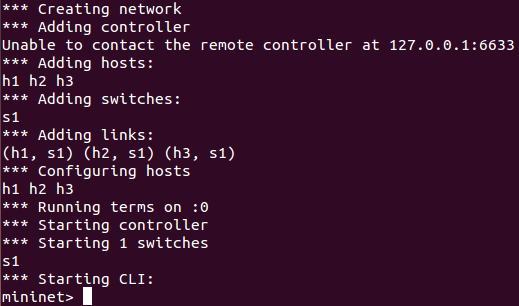
\includegraphics[width=0.40\textwidth]{./pictures/mininet.png}
	\caption{Mininet start}
	\label{x}
	\end{center}
\end{figure} 

\subsection{OpenFlow}
Hier teilen wir der Bridge mit welche OpenFlow Version verwendet werden soll. Dieser Befehl muss auf s1 ausgeführt werden. 
\begin{lstlisting}
ovs-vsctl set Bridge s1 protocols=OpenFlow13
\end{lstlisting}

\subsection{Ryu application starten}
Nachdem die Vorbereitungen getroffen wurden, können wir jetzt Ryu starten mit dem erstelltem Script als Parameter. Dieser Befehl muss auf dem erstelltem Controller c0 ausgeführt werden. 
\begin{lstlisting}
ryu-manager --verbose simple_hub_v2.py
\end{lstlisting}
\begin{figure} [H]
	\begin{center}
	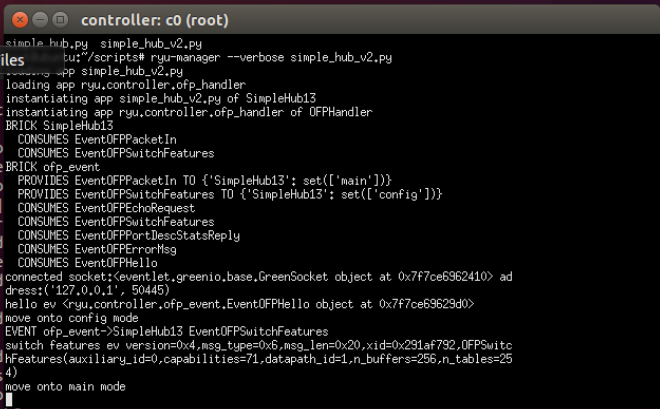
\includegraphics[width=0.50\textwidth]{./pictures/ryu_start_simple_hub.png}
	\caption{Ryu application start}
	\label{x}
	\end{center}
\end{figure} 

\subsection{Traffic}
Nachdem alles gestartet wurde können wir im Mininet von Host (h1) zu Host (h3) pingen um zu sehen ob der Verkehr mittels OpenFlow fliesst. Der Verkehr können wir mit Hilfe von Wireshark sniffen. Der gesamte Traffic verläuft über den Controller c0. Jedes Paket wird in ein OpenFlow Paket gekapselt und weitergeleitet. Der Hub ist nicht in der Lage einen Flow zu lernen. 
\begin{figure} [H]
	\begin{center}
	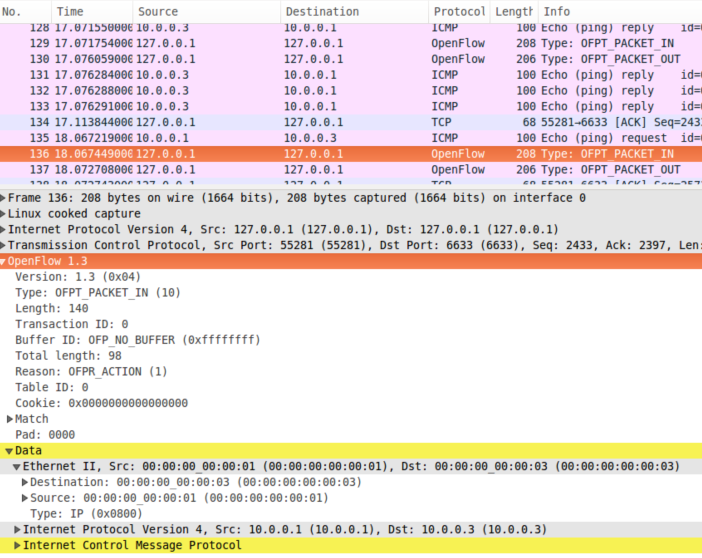
\includegraphics[width=1.00\textwidth]{./pictures/simple_hub_traffic.png}
	\caption{Mininet Traffic ping from h1 to h3}
	\label{x}
	\end{center}
\end{figure} 


\end{document}